\documentclass[tikz]{standalone}
\begin{document}
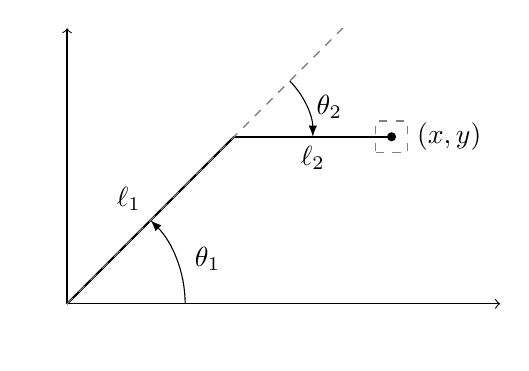
\begin{tikzpicture}
  %\draw[help lines] (-0.5, -0.5) grid (5.5,3.5);
  %\node [below] at (5.5,0) {$x$};
  %\node [left] at (0,3.5) {$y$};
  %\node [below] at (1,1) {$y=x$};
  % \node [above] at (4,1.25) {$y=1 + 1/x$};
  \draw [<->] (0, 3.5) -- (0, 0) -- (5.5,0);
  \begin{scope}
    \clip (-0.5,-0.5) rectangle (5.5,3.5);
  %\draw[thick, domain=0.05:5.5, samples=100] plot (\x, {1 + 1/\x});
  %\draw[thick, domain=0:5.5] plot (\x, {\x});
  \draw [dashed, gray] (0,0) -> (6,6);
  %\draw [dashed, gray] (3,0) arc [radius=3, start angle=0, end angle= 90];
  %\draw [dashed, gray] (2+2.1213203435596424,2.1213203435596424) arc [radius=2, start angle=0, end angle= 360];

  \node [above left] at (2.1213203435596424/2,2.1213203435596424/2) {$\ell_1$};
  \draw [thick] (0,0) -> (2.1213203435596424,2.1213203435596424);
  %\draw [<->] (0.2,-0.2) -- (2.1213203435596424+0.2,2.1213203435596424-0.2);

  \node [below] at (2.1213203435596424 +1,2.1213203435596424) {$\ell_2$};
  \draw [thick] (2.1213203435596424,2.1213203435596424) -> (4.1213203435596424,2.1213203435596424);
  \draw [fill] (4.1213203435596424,2.1213203435596424) circle [radius=0.05];
  \draw [dashed, gray] (4.1213203435596424 - 0.2,2.1213203435596424-0.2) -- (4.1213203435596424+0.2,2.1213203435596424-0.2) -- (4.1213203435596424+0.2,2.1213203435596424+0.2) -- (4.1213203435596424-0.2,2.1213203435596424+0.2) -- cycle;
  \node [right=0.2cm] at (4.1213203435596424,2.1213203435596424) {$(x, y)$};

  \draw [->, -latex] (1.5,0) arc [radius=1.5, start angle=0, end angle= 45];
  \node [right] at (1.5,0.5740251485476346) {$\theta_1$};
  %\draw [dashed, gray] (2+2.1213203435596424,2.1213203435596424) arc [radius=2, start angle=0, end angle= 360];
  \draw [->, -latex] (2.8284271247461903, 2.8284271247461903) arc [radius=1, start angle=45, end angle= 0];
  \node [right] at (3.04519987607093, 2.504003775924732) {$\theta_2$};


  \draw [dashed, gray] (0,0) -> (6,6);

  \end{scope}


\end{tikzpicture}
\end{document}
